\section{Experiment 1: Quadratic Voting, Likert scale surveys and Donation}
\subsection{Methodology} \label{method-1}
The first experiment aims to answer research questions one and three. 
We collected 213 valid submissions from Mturk in 2020. %actual 216, screens 3.4K 
%Participants were recruited to match the US 2019 census for education level and age.
Participants were told that this study aims to understand their opinions toward societal causes and will be asked to complete a donation task.
Participants received \$0.75 and \$1.75 according to the groups they are assigned to.

\begin{figure}[htpb]
    \centering
    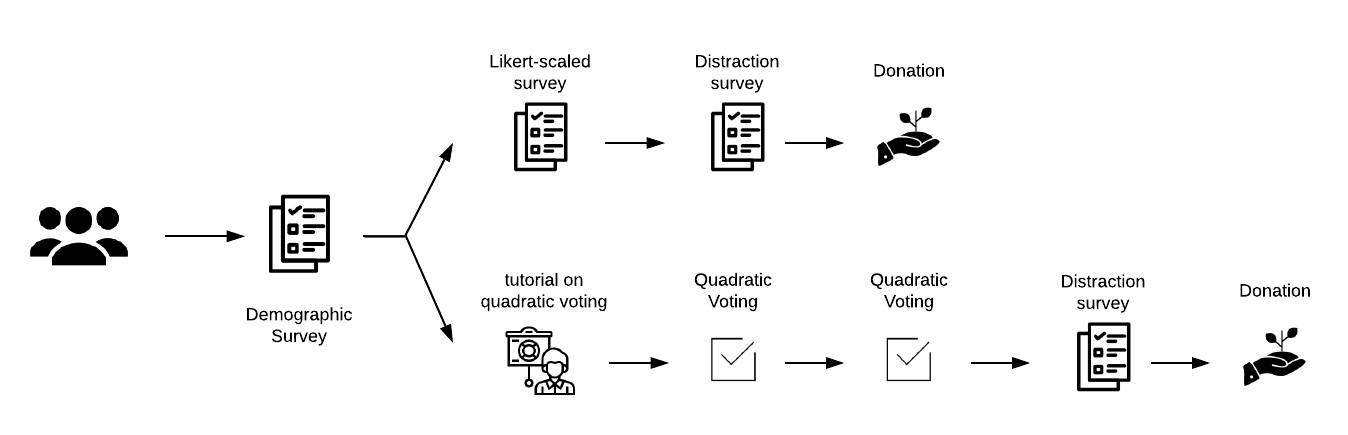
\includegraphics[width=\textwidth, keepaspectratio=true]{content/image/exp1_flow.png}
    \caption{
        Experiment one conducted between subjects. Participants were divieded into two groups. Participants that took the upper path is the Likert Group and the alternative is the QV group.
    }
    \Description[Image describing the flow for experiment 1]{Image describing the flow for experiment 1}
    \label{fig:exp1_image_flow}
\end{figure}

To answer research question one, we first want to see if people donate honestly with the opinion one indicated in the survey.
Donation is a real-life behavior that has immediate and direct monetary impacts.
Not only is donation easy to conduct online and large scale, but it is also reflected directly to the participants.
Donation tasks were used in many experiments \cite{Xiao2019, benz2008people, gendall2010effect} as an effective indicator of participants' behavior.
At a high level, we experimented with the flow shown in Graph \ref{fig:exp1_image_flow}.
All participants first filled out the demographic survey.
Then they will complete some form of opinion collection (the yellow box), followed by a distraction survey.
Finally, participants will do a donation task.
We explain each section in detail.

In the demographic survey, we collected the participant's gender, ethnicity, age range, household income level, education level, current occupation.
We made sure that each of the seven groups followed the US 2019 census containing participants with the same proportion in age and education level.
The first group, known as the Likert group (Upper path in Graph \ref{fig:exp1_image_flow}), will reveal their opinion using a Likert scale survey.
The second to the seventh group of participants, the QV group (Lower path in Graph \ref{fig:exp1_image_flow}), will reveal their preference by completing two QVs with different numbers of voice credits successively.
The reason why we further divided these participants into group two to seven, is to answer research question three, that is whether the number of voice credits impacts the outcome.
These two voice credits that participants experience are drawn from three possible values: $N \times O$, $N^1.5 \times O$, $N^2 \times O$, where $N$ is the number of options in the survey, and $O$ is the number of levels, excluding neutral on the Likert scale survey. %not sure if this is clear
In our case, with nine options and used a five-point Likert scale survey, the three values would be $36$, $108$, and $324$.

% Explain text: On a 5-point Likert scale, users can vote at most two levels, positive or two levels negative (and a neutral). We want to make sure that in a QV, the users have enough budget to cast two votes either positively or negatively for all options, similar to the Likert survey (so that we are not over limiting their ability to express the same intensity in QV). In QV, two votes cost four credits. So, the minimum number of total voice credits is 4 * # of options = 4*9 = 36. To test how larger budgets impact people's choices, we set an exponential increase in the total voice credits based on the number of options. In the minimum case, we use (# of options)^1. We scale the budget as (# of options)^1.5 and (# of options)^2 in the second and third budgets. Hence, the second budget is 4 * (# of option)^1.5 = 4 * 27 = 108. The third budget is 4 * (# of option)^2 = 4 * 81 = 324.

In the Likert group, the survey looks like a typical five-point Likert scaled survey.
Participants were presented with nine societal causes, and were asked the importance each of these causes: From ``Very important'' to ``Very Unimportant.''
In the QV group, participants were asked to watch a prerecorded tutorial video of QV's concept and how to operate the QV interface.
Participants are granted unlimited time to interact with a demo QV interface. 
This process is shown as ``tutorial on quadratic voting'' in Graph \ref{fig:exp1_image_flow}.
To ensure that participants paid attention to the video and understood QV, they were asked to answer at least three of the five multiple-choice questions correctly to continue with the survey.
Participants would vote for the same causes.

Once participants completed their surveys in the opinion collection stage, they were asked to finish a series of short answer questions allowing them to express their thoughts related to another set of societal issues.
We called this survey the distraction survey because it is designed to prevent participants from connecting their survey responses to their final donation task.

We ask participants to perform a donation in the final stage. 
To ensure the incentive compatibility of the design, participants do not donate imaginatively.
Participants are aware that every one in 70 participants would win 35 US dollars.
Assuming winning the 35 US dollars, the participants were asked if they would want to donate some money to some of the nine charity groups.
Participants are also aware that they keep the remaining amount of undonated money if they win the lottery.
Further, participants are aware that the research team will match one dollar to each one dollar they donated to an organization. 
This setup means the donation carries a cost.

To minimize the difference across the study, we use the same prompt across Likert scaled survey, QV, and the donation task.
We explicitly tell the participants that there are limited resources in the society, and people have different preferences in how resources should be allocated and ask the participants, ``What societal issues need more support?''
The nine societal causes cover a broad spectrum of categories.
We used the categorization of charity groups on Amazon Smile, a popular donation website that has accumulated over 100 million dollars of donations as our topics of the societal causes.
The categories include (1) Pets and Animals, (2) Arts, Culture, Humanities, (3) Education, (4) Environment, (5) Health, (6) Human Services, (7) International, (8) Faith and Spiritual, and (9) Veteran. 
Within each of these categories, we select one charity from Amazon Smile as the representation of the subject matter used in the donation task.

\subsection{System Design}
We using Python Flask for the back-end, Angular for front-end, and MongoDB for database storage to construct the voting system. 
The experiment source code is publicly available \footnote{Not yet public}, and so is the QV interface as a stand-alone repository \footnote{https://github.com/hank0982/QV-app}.

\begin{figure}[htpb]
    \centering
    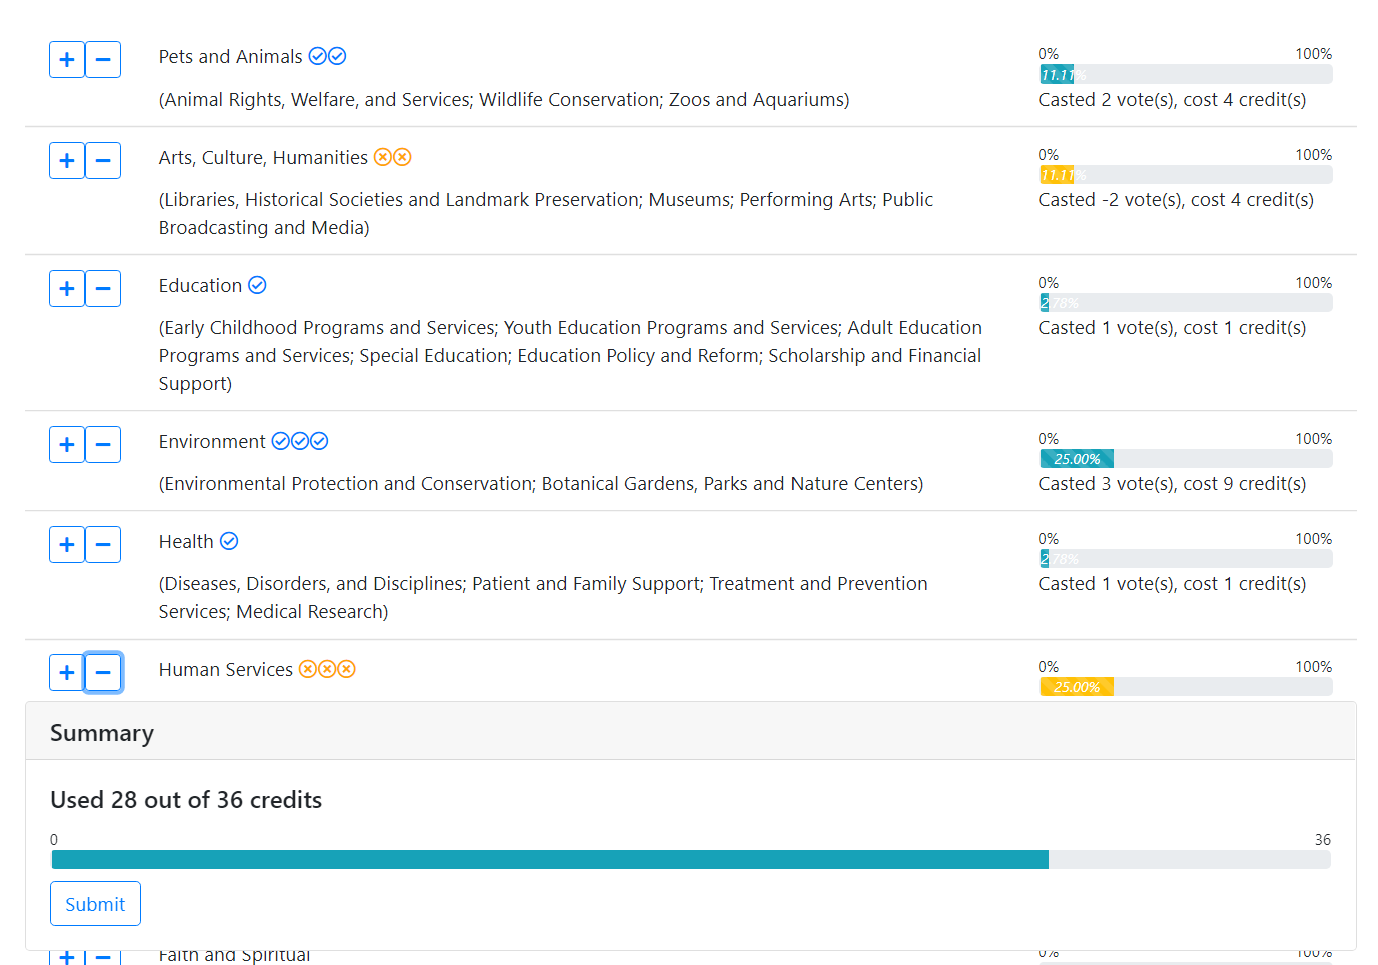
\includegraphics[width=0.7\textwidth, keepaspectratio=true]{content/image/qv-donation.png}
    \caption{
        The QV voting interface used across both experiments. Through mutiple iteration of design, the interface allows participants to vote, and provide some information about how their votes were allocated. The progress bar implementation were inspired by knapsack voting interface by \textcite{goel2015knapsack}.
    }
    \label{fig:qv_donation}
\end{figure}

The QV interface, is shown in Figure \ref{fig:qv_donation}.
We omit the prompt on the top of the interface.
The body section is the voting panel, containing all options to vote for.
To the left of the options, participants vote using the plus and minus buttons.
Buttons are disabled if the number of voice credits does not permit the next vote.
A bar on the right of the option shows the proportion of voice credits used to that option with text associated with the visual.
The different colors and the icons to the right of each option exhibits for or against that option.
The summary panel always floats at the bottom of the page to ensure visibility.
A progress bar shows the number of voice credits that the participants have and had not used.\par